\chapter{Development Process}
%%%%%%%%%%%%%%%%%%%%%%%%%%%%%%%%%%%%%%%%%%%%%%%%%%%%%%%%%%%%%%%%%%%%%%%%%%%%%%%%%%%
Since I was working by myself on this project, I did not adopt 
a formal development process, 
but my development process has been iterative, with continuous deliveries, 
and continued improvement. The nature of this project is very modular:
it consists of various algorithms which do not rely on one another.
Thus I worked on each algorithm individually 
from conception to completion, published it to the live website 
and then I moved on to the next algorithm. 
The process of creating an AV for a given problem went (roughly) as follows:
\section{Choose which Algorithms to Cover}
\hspace{-0.26in}
I selected from the set of problems taught in Comp 482 at CSUN because
the goal of this project is to create a tool to be used by CSUN faculty.
I wanted to create an AV for at least one of each major section
(Greedy, Divide and Conquer, Dynamic Programming, Network Flow)
taught in that class, but due to time constraints I had to narrow it down even further.
I chose the AV's based on how much it would improve a lecturer's ability to 
communicate the problem and its solution,
how important the topic is for learning other lessons, 
and how tedious it is to solve the problem without the use of an AV. 
In \textbf{Chapter \ref{the-algorithms} The Algorithms}, I discuss in detail why 
I chose each of the algorithms that I created an AV for. 
%
\section{Set the Scope and Limitations}
\hspace{-0.26in}
I was often faced with a decision between making an AV more general-purpose
versus one that would accomplish a specific task very well. 
I kept the goal of this project in mind when making such a decision 
(which almost always turned out to be the less generalized option). 
Thus I imposed a set of restrictions in scope and problem size
in order to improve the ability of each AV to accomplish its task. 
\newline\newline
These restrictions ensure that the app runs smoothly on classroom computers, 
fits nicely onto a web page, 
and does not overwhelm the viewer with too much information. 
However, I made sure the app would allow instances that were much larger than 
what a lecturer could show by hand. 
For example, a typical Stable Marriage problem that is demonstrated in lecture 
will have no more than 3 men and 3 women.
Meanwhile the Stable Marriage AV in my project allows for as many as 14 
(but I recommend keeping it below 7).
\newline\newline
I also limited the scope of each problem to the simplest version that is 
covered in a typical class. The reason for this is to have the app be easier to use. 
%
\section{The Data Model}
\hspace{-0.26in}
The first part of creating each AV is creating the data model. 
The data model consists of 
data structures (arrays, maps, lists, etc.)
that represent an instance of the problem, 
and functions that mutate those data structures as an algorithms is being performed. 
Although most problem instances can be represented with just one or two data structures, 
the data model of an AV also includes other data structures that 
provide different perspectives of the instance and others that are necessary for the solver.
For example, the Stable Marriage data model includes: 
\begin{itemize}
	\item Two $n \times n$ arrays that show preference lists, 
	\item A list of $length \leq n$ that shows Tentative Matches, 
	\item Two lists of $length \leq n$ that show any people who are currently unmatched. 
\end{itemize}
The only \textit{necessary} data structure in the above list is the first two, 
but the third one provides utility that makes the code easier to write and follow.
\newline\newline
Since this project focuses on AV's to be used in lecture, 
the problem instances don't become large enough for 
memory management, efficiency, and response time 
to become an issue. 
And since the app is programmed in JavaScript, 
a language with weak typing (almost no typing), most of the data structures 
consisted of either arrays or objects.
%
\section{The \textsc{Instance Maker} and Save/Load}
\hspace{-0.26in}
The Instance Maker of an AV consists of all the parts of the user interface 
that allow the user to create and edit instances of the given problem. 
The first step of creating the Instance Maker is to create a textbox, 
even though it almost always gets removed from the final version of the Instance Maker 
(because typing into a textbox is very dull and prone to errors). 
But having a reliable way to test various inputs is useful when determining
which user interface components (buttons, sliders, or custom components) to implement.
\newline\newline
I prioritized components that are easy to use, 
because it is important for lecturers to use as little time as possible
creating problem instances (that's one of the goals of this project after all)
which will allow them to spend more time explaining the algorithm and how it works. 
\newline\newline
Depending on the specific algorithm, an Instance Maker requires one or more of 
the following functionalities:
\begin{itemize}
	\item Create a new piece of data in the Data Model. 
		\subitem For example: adding a new interval in Interval Scheduling
	\item Remove a piece of data from the Data Model.
		\subitem For example: removing an interval from Interval Scheduling
	\item Edit a piece of the Data Model.
		\subitem For example: reordering a person's preference list in Stable Marriage.
\end{itemize}
A few of the more specific Instance Maker components will be discussed in \textbf{Chapter \ref{guide} Guide}.
\newline\newline
The last step in creating the Instance Maker is the Save/Load specified in 
Requirements \ref{req-load} and \ref{req-save}.
The Save/Load feature converts the most important parts of the Data Model into text. 
The purpose of the Save/Load feature is 
to further reduce the amount of time lecturers spend creating instances in class
by having them load up instances that they have created in advance.
I chose text files to make this feature as easily accessible as possible. 
%
\begin{figure}[ht]
	\centering
	\caption{Sequence of Development}	
	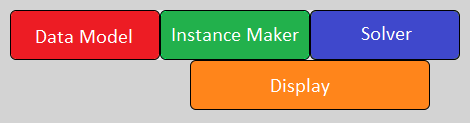
\includegraphics[height=1.25in]{images/development-process-timing.png}
	\label{fig-develpoment-process-timing}
\end{figure}
\section{The \textsc{Display}}
\hspace{-0.26in}
The Display was often developed in parallel to the Instance Maker because 
the very nature of creating interactive diagrams requires the user 
to be able to interact with the diagrams. 
Oftentimes the line between the Instance Maker and the Display gets blurred, 
and they become a single entity. 
Furthermore, the Display also needs to be developed in parallel to the 
Solver (see below) because it needs to react to the Solver and 
update as an algorithm is being performed (see Figure \ref{fig-develpoment-process-timing}). 
\newline\newline
Creating the Display means taking the most interesting parts of the Data Model and 
turning them into pretty, visual diagrams. 
When creating displays for the various problems I thought about the way
each of these problems are solved on the whiteboard during lecture, 
on paper for homework, and also on paper for tests.
I attempted to create visuals that matched (some of) those scenarios 
in the hopes that it will give students an idea of how to approach their assignments. 
%
\section{The \textsc{Solver}}
\hspace{-0.26in}
The final and most difficult part of each problem is the Solver. 
The Solver is responsible for implementing the algorithm,
but it must do so in a stepwise manner. 
It is important to determine what constitutes a single ``step'' in the Solver, 
where a step corresponds with a single action by the user. 
Having each step be too small would force the lecturer to spend more time 
interacting with the Solver than their own students, while having each step be 
too small would give the students a hard time understanding what's going on. 
An appropriate size for each step is one or two lines of the algorithm's pseudocode.
\newline\newline
The reason why the Solver is the hardest part of the development process is because
its accuracy is extremely important. 
Having the Solver produce an incorrect result would completely negate 
any benefits of the entire app.
%See \textbf{Chapter \ref{testing} Testing and Validation} for more information about testing.
\newline\newline
Although the actions of the Solver are represented in the Display, it is often 
useful for the Solver to provide a second form of feedback through messages. 
These messages often narrate what is being done with each user interaction, 
and their language is similar to the pseudocode of the algorithm. 
